\section{活動編輯}

\begin{frame}{活動編輯}
\begin{itemize}
\item 上火車之後忘了停錶
\item 想獨立出畫圖的那段活動(比如把騎去泰北高中以及從泰北高中騎回宿舍的部份從神掌的活動中獨立出來)
\item 想獨立出比賽的那段活動(比如開賽前$10$秒就會先按錶,但是那$10$秒影響了 Strava 上看到的成績)
\item 計時失敗
\item 想把畫圖騎錯路的地方刪掉
\item 活動分成了兩段紀錄,想合併成一個活動(比如騎到助航站之後很興奮就先上傳活動了,回去之後想把去程與回程的合併在一起)
\end{itemize}
\end{frame}

\begin{frame}{Strava 內建功能(網頁版)}
\begin{multicols}{2}
\begin{itemize}
\only<1>{
\item 點三個點$\to$Crop/Split
\item Crop:裁切
\item Split:分割
\newpage
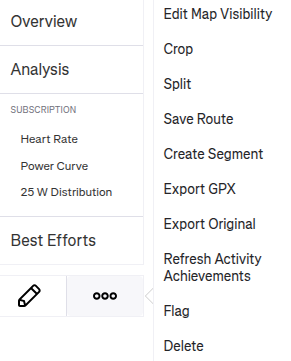
\includegraphics[height=6cm]{cropSplit.png}
}\only<2>{
\item 裁切:去頭去尾\\
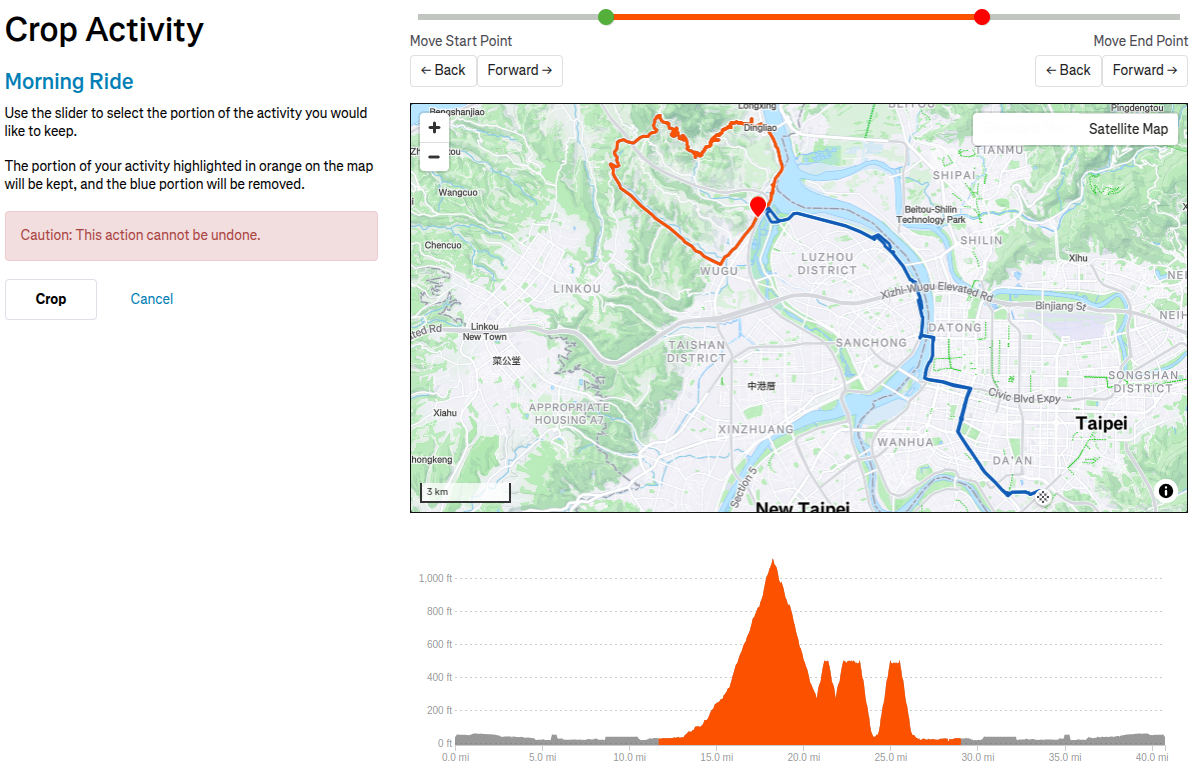
\includegraphics[width=7cm]{crop.png}
\newpage
\item 分割成$2$或$3$個活動\\
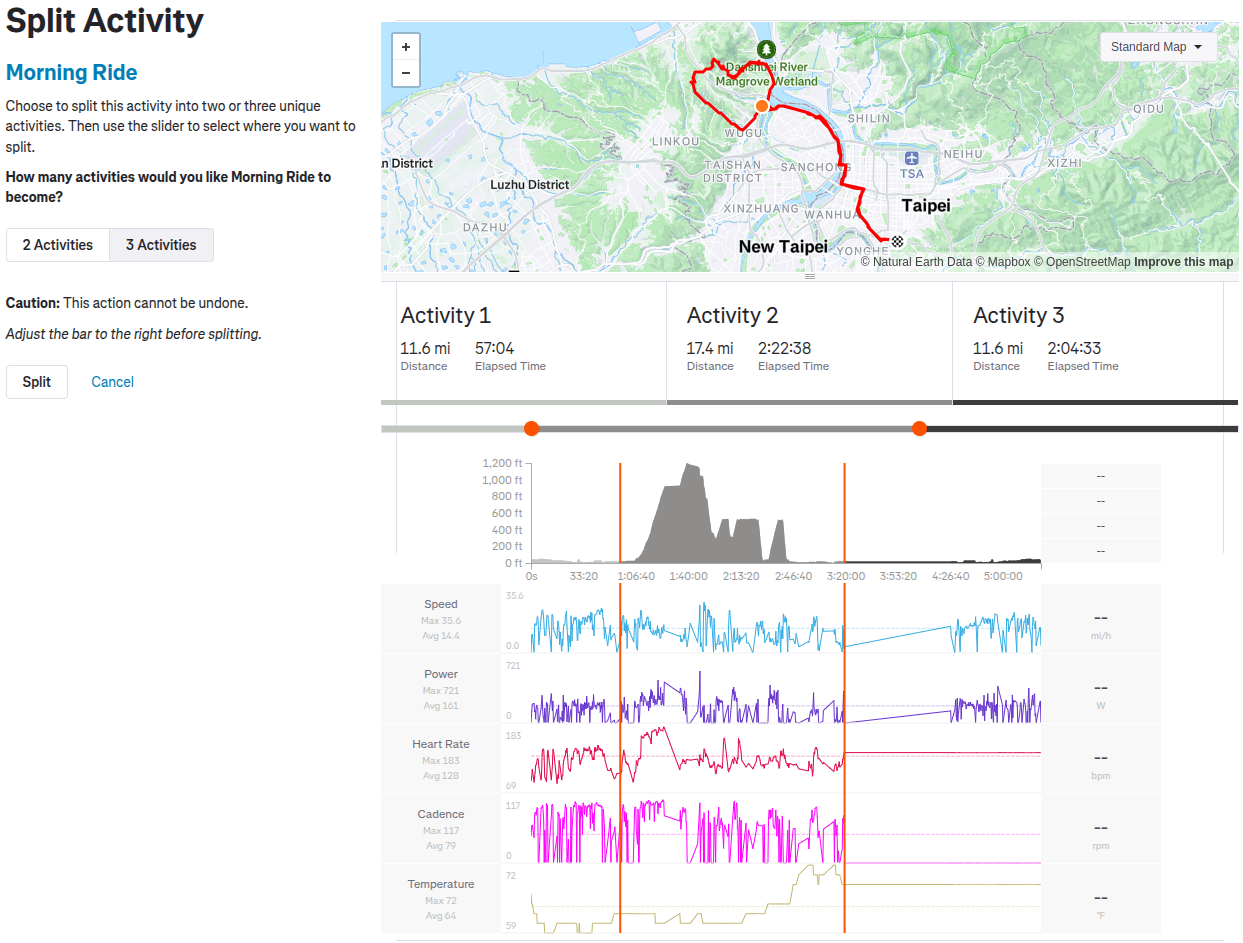
\includegraphics[width=7cm]{split.png}
}
\end{itemize}
\end{multicols}
\end{frame}

\begin{frame}[fragile]{合併活動(網頁版)}
\begin{multicols}{2}
\begin{itemize}
\item 點三個點$\to$Export GPX/Export Original\\
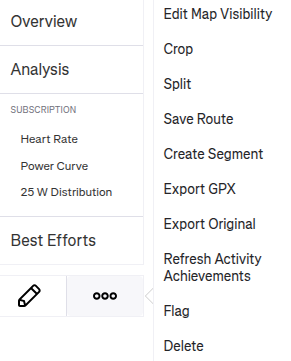
\includegraphics[height=5cm]{cropSplit.png}
\item .fit:使用\href{https://www.fitfiletools.com/#/top}{這個網站}
\item .gpx, .tcx, .csv:使用\href{https://gotoes.org/strava/}{這個網站}
\item 常見問題:功率/心率資料遺失(未知原因)
\end{itemize}
\end{multicols}
\end{frame}

\begin{frame}{GPX 檔}
\begin{itemize}
\item Strava 用來儲存一個活動的檔案格式
\item 車錶通常是 .fit 格式,上傳 Strava 會自動轉成 .gpx
\item 與 .xml 有相近的格式,可以使用 .xml 相關的 parser 來處理(例如 Python 的 \href{https://docs.python.org/3/library/xml.etree.elementtree.html}{xml.etree.ElementTree} )
\item Meta data 與單個紀錄點(需注意 namespace 的處理):\\
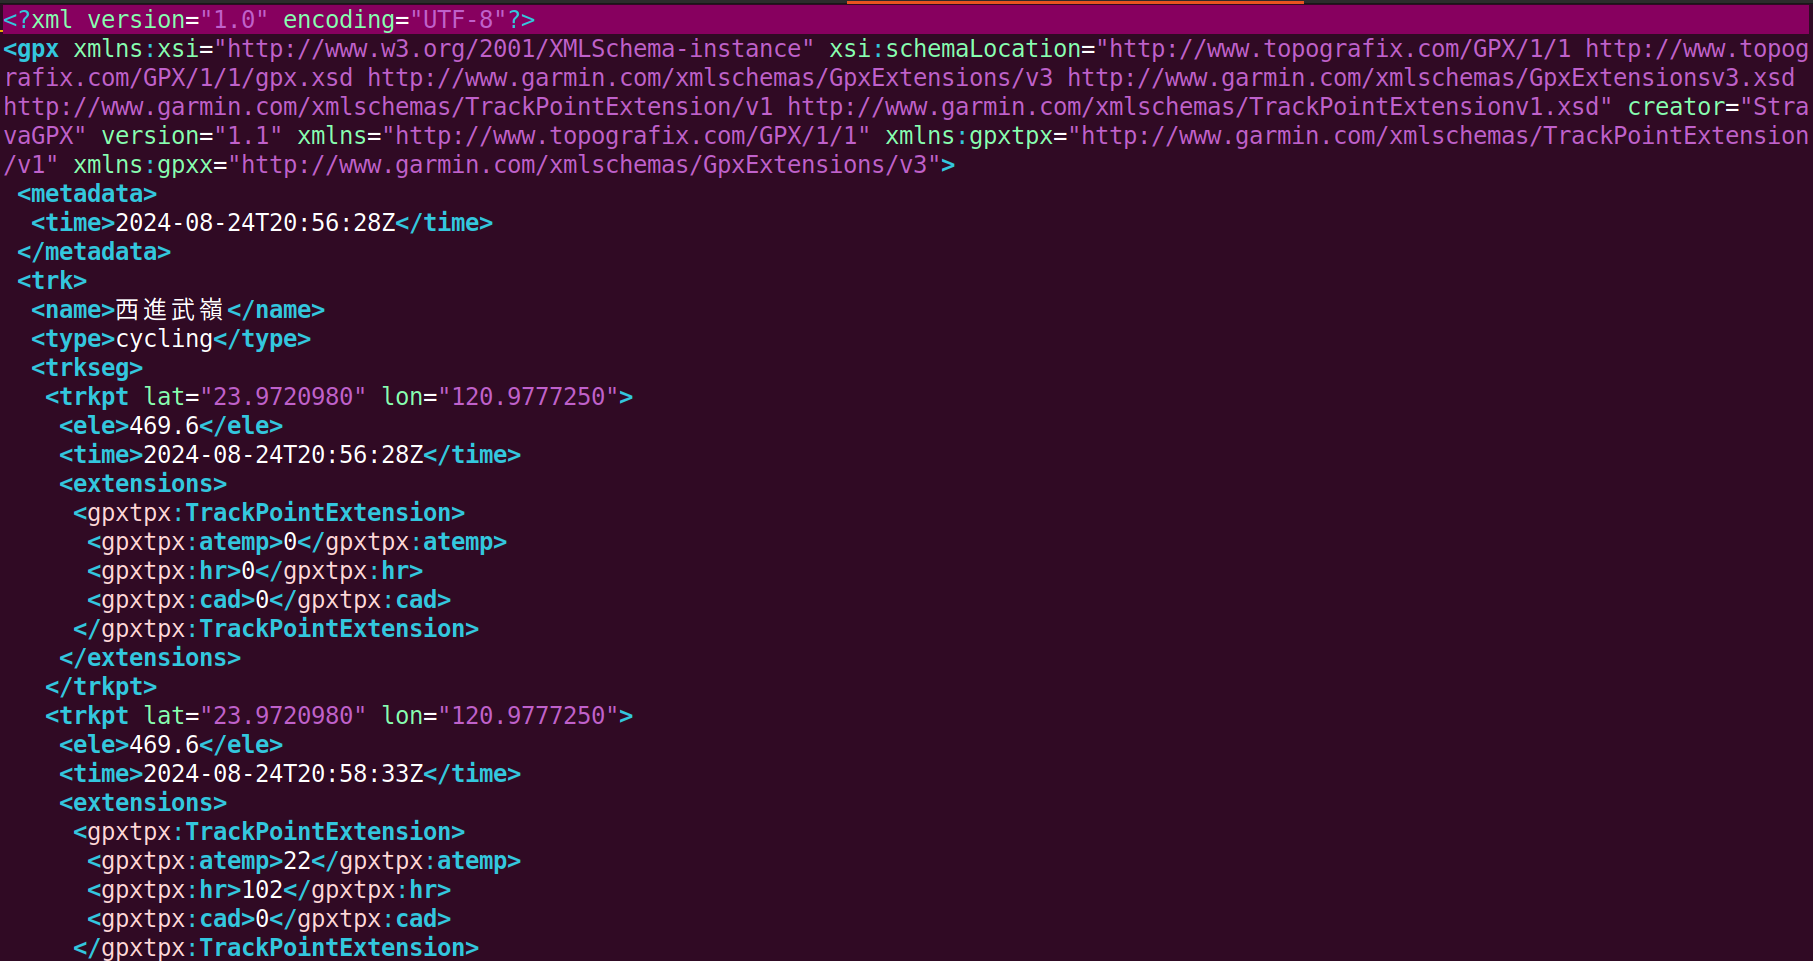
\includegraphics[width=7cm]{gpx1.png}
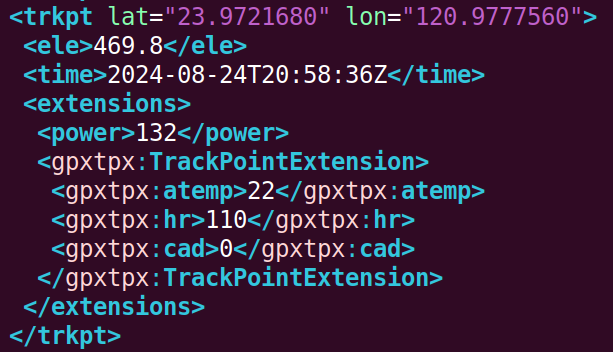
\includegraphics[width=7cm]{gpx2.png}
\end{itemize}
\end{frame}

\begin{frame}{合併活動}
\begin{itemize}
\item \href{https://github.com/brianhsu7476/activityEditPublish}{工具(持續更新中)}
\item 
\end{itemize}
\end{frame}
